\subsection{Topic Models}

\begin{figure}[!h] 
	\centering 
	\includegraphics[scale=0.3]{figs/lda.eps}
	\caption{Bayesian Network of Latent Dirichlet Allocation} 
	\label{fig:lda_pgm}
\end{figure}

Topic models are useful statistical models for finding the topics in a corpus.
It has been used to summarize topics in academic papers
\cite{griffiths2004finding}, automatically tag documents, find aspects in
online reviews from Amazon and Yelp \cite{Jo2011}, etc.

Latent Dirichlet Allocation (LDA) is one of the most popular topic model.
\figref{fig:lda_pgm} shows the Bayesian network of the LDA model. The
generative process of the LDA model is as follows. For each topic $k$, a word
distribution $\phi_k$ is chosen from $Dir(\beta, V)$.  $Dir(\beta, V)$ is the
symmetrical Dirichlet distribution of dimension $V - 1$ and parameter $\beta$,
which is a multivariable probability distribution over the space of the space
of all probability mass functions with domain size $V$.  For each document $i$
in the corpus, a topic distribution $\theta_i$ is chosen from $Dir(\alpha, K)$
and for each word $j$ in the document $i$, a topic $z_{ij}$ is chosen from the
topic distribution $\theta_i$ and finally, the word $w_{ij}$ is sampled from
corresponding word distribution $\phi_{z_{ij}}$.  The Bayesian network has the
following joint probability:

{\footnotesize 
\begin{align*} 
	&\mathrm{Pr}(\theta, \phi, z, w) = \\ 
	&\prod_{k=1}^{K}
	\mathrm{Pr}(\phi_k;\beta) \prod_{i=1}^{M} 
	\mathrm{Pr} (\theta_i;\alpha) \prod_{j=1}^{N}
	\mathrm{Pr}(z_{ij}|\theta_i) \mathrm{Pr}(w_{ij}|z_{ij}, \phi) 
\end{align*} 
}

Summarizing the topics in a corpus is one of the main applications of LDA.
Suppose that we have a number of online reviews as input and we want to
summarize two topics from the input. First we can infer the posterior
topic-word distributions $\phi$, which are two Dirichlet distribution with
parameters $\alpha_1$ and $\alpha_2$. Then we pick several words with highest
weights to produce two lists of representative words. Suppose these documents
are online reviews of restaurants and electronic products. If we pick the top
3 words with highest weights in the parameters of the posteriors to represent
the topics, topic 1 may be cooking, taste, service, while topic 2 may be cpu,
performance, price. Thus we find that topic 1 is about restaurants while topic
2 is about electronic products.

Another application of LDA is to add tags to the documents by inferring the
posterior document-topic distributions. In the previous example, an article
can be considered to be related to retaurants if the posterior topic
distribution of the document have higher weight in topic 1 than 2.

Other topic models that are specific to variaous situations are constantly
proposed. The Sentence LDA (SLDA) model assigns only one topic to words in a
sentence to account for the relative positions of words. The Dirichlet
compound multinomial LDA (DCMLDA) model \cite{Doyle2009} uses different
topic-word distributions in each document instead of global ones to account
for the burstiness in a corpus. 


%\small
%\begin{align*}
%	&\mathrm{Pr}(\phi, \theta, z|x) = \\
%	&\frac{
%	\prod_{k=1}^{K} g(\phi^{(k)}; \vec{\alpha}) \prod_{i=1}^{|D|} g(\theta_D;
%	\vec{\beta}) \prod_{j = 1}^{|D_i|} \theta^{(z_{ij})} \phi^{(z_{ij})}_{x_{ij}}
%	}{
%		\int \prod_{k=1}^{K} g(\phi^{(k)}; \vec{\alpha}) \prod_{i=1}^{|D|}
%		g(\theta_D; \vec{\beta}) \prod_{j = 1}^{|D_i|} \theta^{(z_{ij})}
%		\phi^{(z_{ij})}_{x_{ij}} \mathrm{d}z \mathrm{d}\theta \mathrm{d}\phi
%	}
%\end{align*}
%\normalsize

%In Bayesian inference, parameters and data are all treated as random
%variables.  In contrast to frequentist approach \KZ{what exactly is
%frequentist approach} (e.g. support vector machine, k-means clustering) where
%parameters are often treated as unknown fixed constants to be learned,
%parameters in Bayesian inference are model as random variables to capture the
%uncertainty in the parameters. Prior distributions are assigned to parameters
%and the inference task is to calculate the full posterior distribution of the
%parameters given the data. The
%
%
%\figref{fig:lda_pgm} is the Bayesian network of the LDA model.  In a bayesian
%network, nodes are constants and random variables which include parameters and
%data. In the case of LDA, $\alpha$ and $\beta$ are the constant
%hyperparameters that control the shape of the Dirichlet priors for
%document-topic and topic-word distributions. The plate notation is used to
%represent a set of repeated random variables, where the number on the
%lower-right corner is the number of repetitions. $\phi$'s in the LDA are K
%global topic-word distributions, while $\theta$'s are the document-topic
%distributions. $z$'s are latent random variables that represent the topic
%assigments of the observed words $w$ in the corpus.  The edges between nodes
%represent the conditional dependencies and nodes that are not onnected are
%conditionally independent. For example, the word $w$ has incoming edges from
%$z$ and $\phi$'s so the conditional probability of $w$ is $p(w|z,\phi)$. The
%joint distribution represented by the graph is 
%
%{\footnotesize \begin{displaymath} P(\theta, \phi, z, w) = \prod_{k=1}^{K}
%p(\phi_k;\beta) \prod_{i=1}^{M} p(\theta_i;\alpha) \prod_{j=1}^{N}
%p(z_{ij}|\theta_i) p(w_{ij}|z_{ij}, \phi) \end{displaymath} }
%
%
%\begin{figure}[!h] \centering \includegraphics[scale=0.3]{figs/tsm.eps}
%\caption{Bayesian Network of Topic Sentiment Mixture} \label{fig:tsm_pgm}
%\end{figure}
%
%The topic sentiment mixture model \cite{Mei2007} is able to extract both
%topics and sentiments from a corpus (e.g. Amazon reviews). The model is useful
%for generating topic-sentiment summarization and helping predict user behaviours.
%Following the same notation, \figref{fig:tsm_pgm} is the Bayesian network of
%the topic sentiment mixture model for sentiment analysis.  Instead of
%assigning only topics to words in a corpus, TSM model generates words from 4
%types of distributions: a background distribution $\phi_{B}$ for common
%English words, K topic-word distributions $\phi_{i}$ as in LDA, a positive
%sentiment distribution $\phi_{P}$ for words that express positive opinions and
%a negative sentiment distribution $\phi_{N}$ for words that express negative
%opinions. The generative process is as follows: first decide according to a
%constant probability $\lambda$ whether the word comes from background
%distribution. If not, choose a topic according to a document-topic
%distribution $\theta_i$. For each document and each topic, there's a
%categorical distribution $\delta_{ik}$ called sentiment coverage decides
%whether the word is a positve, negative or neutral word, which is indicated by
%the random variable $s_{ij}$.  Then the word is drawn from the corresponding
%word distribution.
%
%After performing inference on the TSM model, we can find an Maximum A
%Posterior (MAP) parameter estimation. With the MAP parameter estimation, the
%TSM model can be used to rank the sentences for the topics using the
%Kullback-Leibler divergence between the language model of the sentences and
%the topic models; or find the sentiment of a sentence by choosing the one that
%has the minimum KL divergence between the language model of the sentence and
%that of the sentiment; or scoring the overall sentiment towards a topic by
%marginalize out the document of the distribution of the sentiment coverages.
%
%Exponential-conjugate Bayesian networks are those that have nodes in
%exponential family and conjugate priors. The exponential family contains
%common distributions like normal distribution, Gamma distribution, Dirichlet
%distribution, categorical distribution and etc. A conjugage prior $P(\theta)$
%to a likelihood function $P(x|\theta)$ is one whose the posterior distribution
%$P(\theta|X)$ is in the same family as the prior distribution. For example, if
%a Dirichlet prior is for a categorical distribution, the posterior is still a
%Dirichlet distribution with different parameters. It's a restricted yet useful
%subset of Bayesian networks, which is used in many applications. More
%importantly, these Bayesian networks can be dealt with by the automated
%inference tools efficiently using variational inference or Gibbs sampling with
%little user tuning. Strictly speaking, the LDA model and the TSM model are not
%in exponential family because they have mixtures of exponential distributions.
%But this problem can be solved by introducing latent variables (e.g. topics
%$z$ in LDA, $b$, $s$, $z$ in TSM). The resulting models are still able to be
%handled by the automated inference tools.
%
%\KZ{can handle arbitrary models and why mllib cannot easily handle them?  put
%pgms of different models (not limited to exponential-conjugate models), need
%applications to justify the need of a PL} 
%
%\ERIC{subsection 1. pgm and models; what are input and queries; subsection 2.
%how to use inferSpark;
%BASELINE solution}
%
%\KZ{move the following to this section}
%For example, the Topic Sentiment Mixture model \cite{Mei2007}, which is used
%to generate topic-sentiment summarization of a corpus (e.g. online reviews)
%and help predict user behaviour, is a Bayesian network that encodes
%dependencies between the latent sentiment and topic variables and the data.
%The topic-sentiment analysis task is done by performing inference on the
%Bayesian network, or in other word calculating the posterior distribution of
%the latent variables given the corpus.


%\subsection{InferSpark Syntax}

%An InferSpark model definition has similar syntax with normal Scala
%class/object definition. It can reside in the same file as other scala code.
%\figref{fig:lda_model} is the model definition of LDA. The model definition
%starts with the ``@model'' annotation, followed by a class definition. The
%class parameters (K, V, alpha, beta) are treated as constants in the model,
%which will be determined at runtime but prior to the execution. The only
%allowed definitions inside the classbody are the definitions of random
%variables prefixed with ``val''.  Ranges represent the plates in Bayesian
%networks. For example, line 3 in the LDA model definition defines a plate of
%Dirichlet variables with size K. Line 4 uses a special kind of range ``?'' in
%InferSpark, which means the size of the plate is unknown at the time of model
%definition but will be inferred from the observed variables. As in line 5 and
%6, random variables mapped from previous declared random variables will share
%the plates. When any one of ``theta'' , ``z'' and ``x'' is declared observed
%by providing an RDD of data, the size of ``?'' in line 4 will be calculated
%automatically. ``?'' syntax also naturally handles the situation where each
%documents have different lengths.  In line 6, Categorical(phi(z)) defines a
%mixture of categorical distributions of phi whose mixture probability is
%$\mathrm{Pr}(z)$.



%\begin{figure}[h]
%\begin{lstlisting}
%def infer(): LDA {
%	val xdata: RDD[Array[Long]] = /* load data */
%	val lda = new LDA(K, V, alpha, beta)
%	lda.doc.x.observe(xdata)
%	lda.infer(nIterations)
%	lda.phi.getResult().map{
%	case (vid, result) =>
%		val words = (0 until V).map{word =>
%			(word, result.pseudoCount(word))
%		}.sortBy(_._2)(math.Ordering.Double.reverse)
%		(vid - lda.phi.baseId, words.take(10))
%	}.collect().foreach(println)
%	lda
%}
%\end{lstlisting}
%\label{fig:lda_inference}
%\caption{Calling Inference API}
%\end{figure}

%\begin{figure}[h]
%\begin{lstlisting}
%def predict(lda: LDA) {
%	/* load data */
%	val xpred_data: RDD[Array[Long]] = /* ... */
%	val ldapred = new LDA(K, V, alpha, beta)
%	ldapred.phi.observe(lda.phi.getResult())
%	ldapred.theta.observe(lda.theta.getResult()) 
%	ldapred.x.inferLengthFrom(xpred_data)
%	ldapred.infer(nIterations)
%	val perplexity = 
%	ldapred.x.makeJoinable(xpred_data).innerJoin(ldapred.x.getResult()).map{ 
%	(_, word, result) => 
%		-Math.log(result.probability(word))
%	}.map(_._2).reduce(_ + _) / ldapred.x.count
%	println("perplexity = " + perplexity)
%}
%\end{lstlisting}
%\label{fig:lda_prediction}
%\caption{Prediction using Inference Result}
%\end{figure}
%
%In some cases, it would be useful to set the size of plate without observe
%the variables (e.g. making predictions using the inference result).
%Line 7 of \figref{fig:lda_prediction} shows how to achieve this. When
%``inferLengthFrom'' is called, the sizes of plates are calculated as if
%``observe'' is called, but the random variable is still unobserved.

%\begin{figure}[!h]
%\footnotesize
%\centering
%\begin{verbatim}
%model TSM(alpha: Double, lambda: Double, 
%          phi_B: Array[Double], beta: Double, 
%          beta_P: Double, beta_N: Double,
%          V: Long, K: Long, D: Long, N: Long) {
%  val phi = (0 until K).map(_ => 
%    Dirichlet(beta, V))
%  val phi_P = Dirichlet(beta_P, V)
%  val phi_N = Dirichlet(beta_N, V)
%  val theta =  (0 until D).map(_ =>
%      Dirichlet(alpha, K))
%  val delta = (0 until D).map(_ =>
%      (0 until K).map(Dirichlet(1, 3)))
%  val b = (0 until D).map(_ =>
%      (0 until N).map(_ => Bernoulli(lambda)))
%  val z = theta.map{ theta =>
%    (0 until N).map(_ => Categorical(theta))}
%  val s = delta.map{ delta =>
%    (0 until N).map(_ => Categorical(delta))}
%  val w = b.zip(z).zip(s).map{case ((b,z),s) =>
%    (0 until N).map(j => Categorical(
%      if (b(j)) phi_B
%      else if (s(j) == 0) phi_P
%      else if (s(j) == 1) phi_N
%      else phi(z(j))))}
%}
%\end{verbatim}
%\caption{Topic Sentiment Mixture in InferSpark}
%\label{fig:TSM_pp}
%\end{figure}
%
%LDA is a well-studied with wide application. Hence, a lot of machine learning
%libraries including MLLib implement collapsed Gibbs Sampler, an efficient
%inference algorithm, for the LDA model. When it comes to the customized models
%like the Topic Sentiment Mixture model (see \figref{fig:tsm_pgm}) for
%sentiment analysis, there is no off-the-shelf libraries to use. The user has
%to derive the formula and implement the algorithm by themselves. But with
%InferSpark, the user simply has to write a simple model definition and call
%the APIs using a dozens of lines.
%
%
%\begin{figure}[!h]
%\begin{verbatim}
%object Main extends Apps {
%  /* load parameters */
%  val w = sc.textFile("hdfs://localhost/corpus.txt")
%  val m = TSM(...)
%  m.w.observe(w)
%  m.infer(qualityEvaluator=f, initialIter=10, iter=100)
%  val posterior_phi_P = m.phi_P.posterior
%  /* ... */
%}
%\end{verbatim}
%\caption{Calling InferSpark API on the TSM model}
%\label{fig:TSM_API}
%\end{figure}
%
%In the scala program, the user can create an instance of a model in the
%same way as creating an instance of a class. Each random variable defined in
%the model is a field of the model object. The user can specify the observed data by
%invoking the obesrve method of the corresponding random variable. In the infer
%method of the model object, the ruse can specify parameters to the inference
%engine or rely on the default behaviour. If the user provides a
%quality evaluator and there is more than one available algorithm, both
%algorithm will be run for some initial iterations. Then the quality evaluator
%will be called to evaluate the qualilty of inference and the inference engine
%will heuristically choose the better one to run to the end.
%
%After the inference is finished, the user could launch 3 types of
%queries about the results: expectation query $E[g(\theta)|X]$, posterior
%parameter query and MAP query. The compiler will inspect the queries in user's
%scala program to determine what algorithms are applicable to the inference
%tasks.
